%!TEX root=Principal.tex
\chapter{RACIOCÍNIO BASEADO EM CASOS}
\label{cap:rbc}

Raciocínio Baseado em Casos (RBC) é uma metodologia utilizada em Inteligência Artificial que constrói e utiliza um sistema de base de conhecimento criado a partir de experiências passadas. Esse tipo de comportamento é basicamente o comportamento que os seres humanos têm ao solucionar problemas similares com diferentes experiências obtidas ao longo de suas vida~\cite{Lopez:2013}.

O RBC tenta encontrar sempre uma solução, igual ou parecida com a situação atual, em sua base de conhecimento. Ao encontrar essa solução ou possível solução, o RBC tenta adapta-la da melhor maneira à tarefa atual. Caso não seja identificado nenhum caso similar ao atual sendo a situação totalmente nova é possível inferir uma sequência de ações para o caso e armazena-la para que possa ser consultado ao longo do seu ciclo de vida~\cite{Lopez:2013}.

A metodologia do RBC apresenta quatro fases principais. Essas fases são apresentadas na figura~\ref{fig:rbcciclo}~\cite{Lopez:2013}.

\begin{figure}[h!]
	\centering
	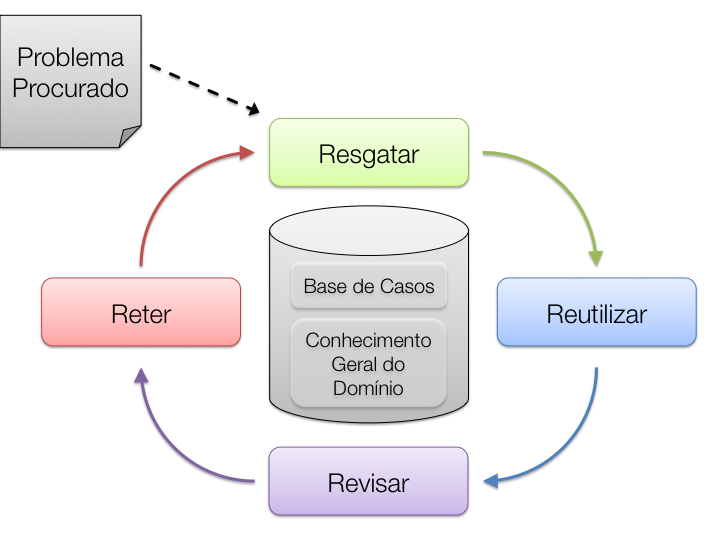
\includegraphics[scale=0.5]{images/cbr-cycle.png}
	\caption{Ciclo da Metodologia de um sistema de RBC.}
	\label{fig:rbcciclo}
\end{figure}

A seguir são apresentadas as fases da figura~\ref{fig:rbcciclo} em detalhes:

\begin{enumerate}
	\item \textbf{Resgatar}: Nessa fase são resgatados casos passados similares ao caso procurado. Métodos indutivos são aplicados normalmente para encontrar os casos armazenados em memória.
	\item \textbf{Reutilizar}: A partir de um conjunto de soluções similares resgatadas formam a base para a construção de uma solução ao problema procurado. A transformação que pode ser obtida nessa fase, ocorre através de generalização e especialização dos casos resgatados.
	\item \textbf{Revisar}: Verificar se a solução apresentada para o problema procurado provem ou não a saída desejada.
	\item \textbf{Reter}: Quando a solução apresenta ao problema gera uma nova experiência, esta pode ser ou não armazenada na base de casos. Para que o armazenamento seja realizado, é confrontado o valor obtido como resposta no processo de revisão do caso, junto com a política de retenção implementada no sistema.
\end{enumerate}

O modelo apresentado na figura~\ref{fig:rbcciclo} é baseado no nível de conhecimento que sistema pode representar. Ele identifica todo o ciclo da metodologia de RBC, do começo ao fim. Esse modelo também é conhecido como 4R’s, pois os nomes dados para cada uma das fases são iniciados com a letra R~\cite{Lopez:2013}.

%%%%%%%%%%%%%%%%%%%%%%%%%%%%%%%%%%%%%%%
\section{Classificação de sistemas de RBC}
\label{sec:classificacaorbc}

Para que sejam construídos, os sistemas de RBC consideram quatro critérios básicos que definem sua topologia~\cite{Lopez:2013}: Fonte de Conhecimento, Função, Organização e Maneira de Distribuição. A tabela~\ref{tab:classificaorbc} apresenta os possíveis tipos para cada um dos critérios.

\begin{table}[h!]
	\centering
	\caption{Classificação de Sistemas de RBC de acordo com sua topologia}
	\begin{tabular}{c | c | c | c} \hline
		Fonte de & Função & Organização & Maneira de \\ 
		Conhecimento & & & Distribuição \\ \hline
		- Textual & - Classificação & - Exclusivo & - Memória Única \\ 
		- Estrutural & - Recomendação & - Níveis Múltiplos & - Memória Múltipla \\
		- Conversacional & - Tutoria & - RBC Híbrido & - Agente Único \\
		- Temporal & - Planejamento & - Meta RBC & - Agente Múltiplo \\
		- Imagens & - Monitoramento & & \\
		& - Gerenciamento de & & \\ 
		& Conhecimento & & \\ \hline
	\end{tabular}
	\label{tab:classificaorbc}
\end{table}

O primeiro atributo apresentado na tabela~\ref{tab:classificaorbc}, Fonte de Conhecimento, refere-se em como é estrutura ou armazenamento do conhecimento passado no sistema. São eles~\cite{Lopez:2013}:

\begin{enumerate}
	\item \textbf{Textual}: É uma coleção de informações em formato de texto, que devem ser lidas pelo sistema afim de identificar a solução do problema. Um exemplo são sistemas do tipo FAQ, que podem ser encontrados em diversas ferramentas e aplicativos.
	\item \textbf{Estrutural}: É definido através de um vocabulário pré definido do problema. Cada caso pode englobar uma quantidade n de variáveis, como por exemplo, um sistema médico que possui informações como idade, histórico de atendimento, índice de massa corpórea, entre outros.
	\item \textbf{Conversacional}: Nesse tipo de RBC o caso é definido maneira iterativa através de um sistema de conversa entre usuários e/ou usuário-sistema, como por exemplo, um sistema de help-desk.
	\item \textbf{Temporal}: Quando os casos possuem uma relação temporal entre si, seja essa relação implícita ou explicita. Um exemplo desse tipo de sistema é o histórico de jogo de um usuário.
	\item \textbf{Imagens}: Cada caso é obtido através do conhecimento extraído na análise das imagens armazenadas no banco de dados. Essa análise ocorre de acordo com alguns fatores relevantes ao domínio do problema e encontrados nas imagens.
\end{enumerate}

O atributo Função refere-se ao objetivo de aplicação do RBC, ou seja, qual o tipo de problema que ele procura resolver. Abaixo a descrição detalhada de cada uma das funções que um sistema de RBC pode apresentar~\cite{Lopez:2013}:

\begin{enumerate}
	\item \textbf{Classificação}: Utilizado geralmente em aplicações onde existe a necessidade de predizer uma classe ou rótulo. Pode ocorrer de duas maneiras: (I) Através da prognosis sendo feita por duas classes, uma positiva e outra negativa; ou (II) Através do diagnóstico sendo feita por um número discreto de classes para predição.
	\item \textbf{Recomendação}: Utilizado para recomendar algum tipo de produto baseado na similaridade das escolhas passadas do usuário.
	\item \textbf{Tutoria}: Utilizado para buscar uma coleção de exercícios de uma determinada disciplina e assim auxiliar o usuário.
	\item \textbf{Planejamento}: Utilizado em duas tarefas normalmente.  A primeira é deixar o planejamento de um processo ou sistema mais eficiente e a segunda tarefa é realizar o raciocínio e aprendizado a nível de planejamento e não a nível da ação de execução como os demais RBC's.
	\item \textbf{Monitoramento}: Utilizado para predizer anomalias de comportamento durante a supervisão de sistemas, principalmente.
	\item \textbf{Gerenciamento do Conhecimento}: Utilizado para fontes de informação e avaliação do conhecimento, não só lembrando da experiência obtida, mas também aplicando esse conhecimento na solução de tarefas.
\end{enumerate}

O atributo Organização refere-se a combinação de RBC para solução de problemas em um mesmo domínio. A Organização também pode ser encontrada como arquitetura do sistema de RBC. As quatro principais são~\cite{Lopez:2013}:

\begin{enumerate}
	\item \textbf{Exclusivo}: Nessa configuração um único RBC é considerado para resolver o problema.
	\item \textbf{Níveis Múltiplos}: Nessa configuração é considerado um determinado número de RBC para solucionar o problema. Uma aplicação desse tipo de arquitetura é a interpretação de imagens.
	\item \textbf{RBC Híbrido}: Essa configuração é aplicada em problemas que necessitam de soluções híbridas ou complementares. Um exemplo de aplicação é o sistema que realiza o diagnóstico de uma doença combinado com outro sistema que realiza o planejamento para o tratamento dessa doença.
	\item \textbf{Meta RBC}: Essa configuração é utilizada quando existe vários sistemas de RBC que necessitam ser aplicados à um único domínio e é utilizado um segundo sistema RBC que verifica qual é o melhor sistema para ser aplicado dado um determinado caso.
\end{enumerate}

É importante ressaltar que o RBC é uma metodologia e não uma tecnologia. Portanto, cada fase dele pode ser resolvida por diversas técnicas de Inteligência Artificial~\cite{Lopez:2013}.

O último atributo que é apresentado na tabela~\ref{tab:classificaorbc} chama-se Maneira de Distribuição. Ele é caracterizado pela maneira como será feita o processamento dos casos. São classificados em dois critérios apenas: (I) Memória ou o número de casos existentes na base de conhecimento; e (II) Forma de distribuição do processamento, sendo possível em um único sistema ou em múltiplos sistemas. Dessa maneira, é obtido quatro possíveis combinações, são elas~\cite{Lopez:2013}:

\begin{enumerate}
	\item Memória Única, Agente Único;
	\item Memória Única, Agente Múltiplo;
	\item Memória Múltipla, Agente Único;
	\item Memória Múltipla, Agente Múltiplo.
\end{enumerate}

%%%%%%%%%%%%%%%%%%%%%%%%%%%%%%%%%%%%%%%
\section{A Base de Casos ou Conhecimento}
\label{sec:basecasos}

A base de casos é formada por quatro fatores principais: (I) Vocabulário; (II) Casos; (III) Medida de Similaridade; e (IV) Adaptação da Solução. Outros fatores podem ser incluídos na base de conhecimento de acordo com a necessidade do projeto ou aplicação. Ao longo dessa seção será discutido como modelar e organizar o caso na base de conhecimento~\cite{Lopez:2013}.

%%%%%%%%%%%%%%%%%%%%%%%%%%%%%%%%%%%%%%%
\subsection{Vocabulário}
\label{sec:vocabulario}

O vocabulário é um conjunto de termos que servem como base na formulação do caso que será inserido na base de conhecimento. Cada termo do vocabulário mantém o mesmo significado, independente da maneira como foi mapeado, para o domínio da aplicação. Em trabalhos mais recentes, verifica-se que não existe uma maneira de compreender um vocabulário sem a utilização de ontologias. Uma ontologia nada mais é que o relacionamento entre as palavras do vocabulário. Esse recurso auxilia a metodologia de RBC de tal forma, que seja possível identificar o relacionamentos entre os elementos de um caso a nível semântico~\cite{Lopez:2013}.

%%%%%%%%%%%%%%%%%%%%%%%%%%%%%%%%%%%%%%%
\subsection{Modelando um Caso}
\label{sec:casemodeling}

Um caso é a instância da descrição do processo que envolve o problema e a solução. Ele precisa descrever de maneira clara o problema e a sua solução de maneira separada e detalhada. Um maneira de representar um caso é através de uma tupla formada por $<p, s, o>$, onde $p$ é a descrição do problema, $s$ representa a descrição da solução e $o$ é a saída espera da aplicação do processo. Existem diversas maneiras de descrever um problema, as principais são através de um modelo atributo-valor ou através do relacionamento entre os objetos. O modelo atributo-valor é mais simples e permite, de acordo com o peso especificado, ignorar alguns atributos na hora do cálculo da similaridade~\cite{Lopez:2013}.

No modelo de relacionamento entre os objetos, os casos são visualizados como um grafo ou uma árvore mostrando a similaridade entre os casos de acordo com o grau do relacionamento. Modelos mais complexos também podem ser utilizados para determinar o caminho do relacionamento. Além disso, séries e sequências também podem ser utilizadas fazendo com que o modelo fique dependente da variável tempo. Quanto aos mapeamentos referentes a solução, geralmente são utilizados algoritmos de predição ou classificação para essa tarefa~\cite{Lopez:2013}.

%%%%%%%%%%%%%%%%%%%%%%%%%%%%%%%%%%%%%%%
\subsection{Medida de Similaridade}
\label{sec:medidasimilaridade}

Geralmente, utiliza-se um algoritmo que efetua a comparação de características de tal forma, que seja possível gerar um grau de similaridade, onde os valores se mantenham entre 0.0 e 1.0. Cada caso armazenado deve possuir um grau de similaridade quando comparado a outro caso da base. Para que o algoritmo chegue a esse valor de similaridade é necessário utilizar duas medidas de similaridade. A primeira medida de similaridade, conhecida como Similaridade Local, refere-se à comparação de uma única característica dos casos. Alguns dos métodos que podem ser usados aqui são~\cite{Gresse:2003}:

\begin{enumerate}
	\item \textbf{Correspondência exata}: Caso as strings sejam escritas da mesma forma. Por exemplo, ``\emph{e-commerce}'' e ``\emph{e-commerce}'' retorna 1.0, enquanto ``\emph{e-business}'' e ``\emph{e-commerce}'' retorna 0.0.
	\item \textbf{Correção ortográfica}: Ponderação entre o número de caracteres que são iguais pelo número total de caracteres. Por exemplo, ``menino'' e ``menina'', a quantidade de caracteres idênticos: 5. Quantidade total de caracteres: 6. Portanto, a similaridade é dada por: 5/6 = 0,83.
	\item \textbf{Contagem de palavras}: Utilizado em textos maiores. Faz um contagem por palavras idênticas nos casos comparados.
	\item \textbf{Taxa do maior \emph{substring} comum}: Taxa entre a maior sequência de caracteres entre os dois casos pelo número total da consulta.
\end{enumerate}

A outra medida de similaridade é conhecida como Similaridade Global. Essa similaridade gera um valor único referente à comparação de todas as características dos casos. Essas características, ou atributos, podem ter pesos, classificando-o como maior importância ou significância no domínio aplicado. Para ter maior eficiência, a busca pode ser feita em uma base de casos indexada o que auxilia os algoritmos de busca dos casos. A equação~\ref{eq:simglobal} apresenta o cálculo do algoritmo \emph{Nearest Neighbour} (vizinho mais próximo)~\cite{Gresse:2003}:

\begin{equation}
	Sim (X, Y) = \cfrac{\sum W_i * sim(q_i, c_i)}{\sum W_i}
	\label{eq:simglobal}
\end{equation}

\begin{flushleft}
	Aonde:
	\begin{enumerate}
		\item $W_i$ é o peso do atributo.
		\item $Sim (X, Y)$ é a similaridade global entre os casos $X$ e $Y$.
		\item $sim (q_i, c_i)$ é a similaridade local entre o atributo $q_i$ de $X$ e o atributo $c_i$ de $Y$.
	\end{enumerate}
\end{flushleft}

Além das medidas de similaridade apresentadas por \citeonline{Gresse:2003}, pode ser utilizados diversos outros métodos para calcular a similaridade local e global entre os casos. Uma medida de similaridade utilizada entre os algoritmos é a distância euclidiana~\cite{Masiero:2013}. Outras medidas de distância também são utilizadas para essa tarefa como a distância de Mahalanobis~\cite{Mahalanobis:1936}. Contudo, outras técnicas também são capazes de determinar o valor da similaridade entre os casos, como no caso da Lógica Nebulosa ou Lógica Fuzzy~\cite{Lopez:2013}.


%%%%%%%%%%%%%%%%%%%%%%%%%%%%%%%%%%%%%%%
\subsection{Adaptação da Solução}
\label{sec:adaptacaosolucao}

Após a definição do caso com a melhor solução de acordo com a similaridade entre os problemas apresentados, é necessário realizar a adaptação da solução do caso. Existem diversas técnicas de adaptação para a metodologia do RBC. \citeonline{Gresse:2003} apresentam a lista a seguir como as principais existentes:

\begin{enumerate}
	\item \textbf{Adaptação Nula}: quando a solução do caso selecionado é a solução do caso buscado.
 	\item \textbf{Adaptação Transformacional Substitutiva}: Quando o caso possui a mesma estrutura, esta adaptação substitui informações baseadas em regras pré-definidas.
	\item \textbf{Adaptação Derivacional}: Obtém informações sobre como um caso foi construído para que outro seja elaborado. Ou seja, nesta adaptação não se utiliza sua solução.
\end{enumerate}

%%%%%%%%%%%%%%%%%%%%%%%%%%%%%%%%%%%%%%%
\section{Revisão dos Casos}
\label{sec:revisaocasos}

Uma solução resgatada não reflete o sucesso do caso, então inicia-se o processo de revisão desta para que seja decidido se essa irá permanecer na base de casos ou se deverá ser descartada. Para que o processo de revisão ocorra são necessárias duas tarefas. A primeira tarefa consiste na avaliação criteriosa da solução dada a partir do processo de reuso. Nessa etapa, caso seja considerada correta, a solução é armazenada na base de casos através do processo de retenção, que será discutido mais a frente~\cite{Gresse:2003}.

A segunda tarefa da fase de revisão é a tentativa de aprimorar a solução para que ela seja correta para o caso em questão. Para que isso seja possível, o sistema ou até mesmo o especialista deve utilizar o conhecimento específico sobre aquele domínio para alterar a solução. Dessa forma, é possível manter os casos dentro da base com todas as possíveis soluções~\cite{Gresse:2003}.

%%%%%%%%%%%%%%%%%%%%%%%%%%%%%%%%%%%%%%%
\subsection{Avaliando a Solução}
\label{sec:avaliandosolucao}

O processo de avaliação de uma determinada solução é dada a partir do uso parcial ou total dela no processo de aplicação em um novo caso similar. Esse processo pode ser realizado pela monitoração dos resultados da aplicação da solução no caso do mundo real, sendo a monitoração automática (através de sensores) ou através da interação do usuário a partir de um retorno sobre o quão válida é a solução para àquele caso~\cite{Gresse:2003}.

Como a avaliação depende da observação da solução aplicada ao novo caso, ela geralmente ocorre em um processo apartado do sistema de RBC como um todo. Isso ocorre, pois, dependendo da situação, a avaliação pode levar alguns meses para que seja totalmente concluída. Um dos motivos é que a avaliação pode depender de um parecer especializado para ser concluída. Nessa situação, o sistema pode manter a solução na base de casos sendo que este deva permanecer com um indicador dizendo que ainda não foi avaliado~\cite{Gresse:2003}.

Um exemplo para a situação onde a solução demora para ser realizada é quando existe um sistema de tratamento médico onde é necessário esperar que a terapia seja concluída para dizer se a solução foi ou não adequada. Esse período pode levar alguns meses para que o resultado final seja alcançado, impactando diretamente no processo de avaliação da solução~\cite{Gresse:2003}.

%%%%%%%%%%%%%%%%%%%%%%%%%%%%%%%%%%%%%%%
\subsection{Corrigindo as Falhas}
\label{sec:corrigindofalhas}

Após o processo de avaliação é possível saber quais pontos da solução que falharam na aplicação ao mundo real ou em uma simulação. Sendo assim, torna-se factível a correção dessas falhas na solução para o caso em questão. A correção das falhas é dada através da explicação extraída no processo de avaliação da solução~\cite{Gresse:2003}.

As explicações das falhas ainda auxiliam na maneira como o sistema irá corrigi-las de acordo com o conhecimento sobre o domínio. No caso das falhas serem corrigidas por um especialista de maneira manual, é recomendado que este realize uma análise de todos os casos com soluções similares para que a falha não ocorra novamente no sistema. Se a correção for realizada automaticamente pelo sistema, esse deve estar programado para revisar todos os casos armazenados na base de conhecimento~\cite{Gresse:2003}.

%%%%%%%%%%%%%%%%%%%%%%%%%%%%%%%%%%%%%%%
\section{Retenção dos Casos}
\label{sec:retencaocasos} 
O processo de retenção de casos nada mais é do que a inclusão de um caso novo na base de conhecimento. A ideia por trás do processo de retenção é sempre armazenar a solução de um novo problema fazendo com que a base de dados esteja sempre atualizada e em constante crescimento. Quanto maior o número de casos armazenados dentro da base, maior é considerado o poder do sistema de RBC na solução de problemas. Essa etapa é dada através de algoritmos de aprendizado de máquina. Um dos algoritmos mais utilizados são os relacionados ao aprendizado baseado em instâncias~\cite{Gresse:2003}. 

O processo de retenção pode ser implementados em um sistema de RBC de três principais maneiras, são elas~\cite{Gresse:2003}:

\begin{enumerate}
	\item \textbf{Sem retenção de casos}: Esse é a implementação mais simples para um sistema de RBC, pois ela não possui a inclusão automática de novos casos na base de dados. Para que seja possível aplicar essa implementação é necessário possuir um conhecimento sólido sobre o domínio da aplicação do sistema. Dessa forma, o sistema não apresentará nenhum problema que já não esteja bem mapeado pelos especialistas. Um exemplo para esse tipo de sistema é uma linha de produção de um determinado modelo de veículo.
	\item \textbf{Retenção de soluções de problemas}: O tipo de aprendizado gerado por essa maneira de retenção é a mais clássica entre os sistemas de RBC. Nesse tipo de implementação toda vez que um problema é solucionado com sucesso, este é transformado em um caso da base de conhecimento. Dessa maneira, é possível expandir o conhecimento sobre um determinado domínio de aplicação do sistema de RBC. A retenção de soluções de problemas pode também armazenar as soluções que não foram satisfatórias para que essas não sejam utilizadas novamente para os problemas similares.
	\item \textbf{Retenção de documentos}: Nesse tipo de retenção o processo ocorre independentemente de um problema estar ou não solucionado. Na retenção de documentos o aprendizado e, consequentemente, a inclusão de novos casos da base ocorre sempre que um novo conhecimento sobre o domínio torna-se disponível ao sistema de alguma maneira. Por exemplo, toda vez que a descrição sobre um novo produto é disponibilizada pelo fabricante ou quando uma agência de viagens recebe informações de novos pacotes para viagens.
\end{enumerate}

O aprendizado gerado através da fase de retenção de casos  é considerada efetiva para o RBC, caso haja um conjunto de métodos bem trabalhado. Esse conjunto de métodos deve ser capaz de extrair conhecimento relevante sobre as experiências passadas, indexar o conhecimento para que seja possível utiliza-lo em um momento futuro e ainda integrar o conhecimento em uma estrutura existente~\cite{Gresse:2003}. Pode-se considerar os principais aspectos da fase de retenção os seguintes tópicos~\cite{Gresse:2003}:

\begin{enumerate}
	\item seleção adequada da informação armazenada em conjunto com os casos;
	\item seleção da estrutura da informação;
	\item seleção da estrutura de índices para buscas futuras na base;
	\item seleção do tipo de integração a ser realizado na estrutura de conhecimento.
\end{enumerate}

Com os principais conceitos de RBC apresentados, serão discutidos na seção~\ref{sec:rbcaplicado} as aplicações de RBC em diversas áreas de pesquisa. Contudo, o principal foco das aplicações estão em Interação Humano-Robô e Robótica em Geral.

%%%%%%%%%%%%%%%%%%%%%%%%%%%%%%%%%%%%%%%
\section{Raciocínio Baseado em Casos aplicado em Robótica}
\label{sec:rbcaplicado}

O desenvolvimento de aplicações para mundos reais são complexas, não sendo possíveis de uma observação completa do cenário e do ambiente explorado, e ainda as decisões, que devem ser tomadas em tempo real pelo agente em tarefa. Além disso, as tarefas executadas pelos agentes podem mudar a qualquer momento fazendo com que este deva mudar e ainda aprender com os novos comportamentos~\cite{Floyd:2011}.

Assim é proposto um \emph{framework} chamado jLOAF (Java Learning by ObservAtion Framework) permitindo que os agentes possam aprender as tarefas no mundo real através da observação do comportamento dos especialistas. Esse \emph{framework} permite a evolução dos agentes em diversos tipos de ambiente e aplicações. Ele faz com que os agentes aprendam o comportamento na execução de uma tarefa sem que se diga qual tarefa deve ser executada~\cite{Floyd:2011}.

Todas as observações realizadas pelo agente durante a interação do especialista com o ambiente são armazenadas com um caso dentro de uma base de conhecimento. Cada caso é representado por um conjunto de ações e reações entre o ambiente e o especialista que será recuperado pelo agente de acordo com a situação que ele irá encontrar no ambiente real~\cite{Floyd:2011}.

Para testar o \emph{framework} foram realizados testes em quatro casos de estudo diferentes aplicados em tarefas como controle de um braço robótico, jogo de futebol simulado e o jogo de Tetris. Os resultados apresentados são interessantes, pois com o \emph{framework} foi possível fazer com que o mesmo agente fosse capaz de aprender os diferentes domínios sem realizar nenhuma alteração no módulo de raciocínio do agente. Entretanto, existem algumas limitações no \emph{framework}, principalmente quando a tarefa é simples e não existe mudança de domínio. Esse tipo de situação inviabiliza o uso dele, que foi preparado para ambientes e tarefas mais complexas~\cite{Floyd:2011}.

Em outro trabalho um algoritmo para jogos baseado em Raciocínio Baseado em Casos para auxiliar no tratamento de fisioterapia para idosos é apresentado por \citeonline{Hansen:2012}. O jogo utiliza um robô móvel que deve desviar-se de uma bolinha que é jogada por uma pessoa. O robô adapta seu comportamento de acordo com as habilidades apresentadas pela pessoa durante o jogo. As habilidades da pessoa são medidas através do comportamento espaço-temporal dela, ou seja, a dificuldade de deslocamento até a bolinha ou o robô.

Os resultados apresentados durante os testes foram robustos e fazem com que o robô seja uma ótima ferramenta para esse tipo de tarefa. A adaptação do algoritmo utilizando RBC demonstrou boas soluções para ajustar os desafios do jogo. Entretanto, quando a pessoa não mantém um padrão de locomoção faz com que o algoritmo falhe na tomada de decisão. Esse é o um ponto que dever ser melhorado para trabalhos futuros~\cite{Hansen:2012}.

\citeonline{Srinivasan:2006} propõem um sistema para gerar estratégias de comportamentos ofensivos e defensivos em um time de futebol de robôs. O sistema é desenvolvido utilizando a metodologia de RBC unido a um classificador Bayesiano. Cada caso da base de conhecimento é descrito como um conjunto de movimentos que representam uma jogada do time. A jogada que será realizada é escolhida com base na similaridade entre a situação de jogo atual com as armazenadas na base de casos.

No trabalho de \citeonline{Srinivasan:2006} a composição dos casos é feita através de um vetor de características composto pela quantidade de jogadores da equipe, e também do oponente, dentro do quadrante onde a bola é localizada, além do fator que determina distância da bola até o gol. O vetor de características é comparado com os casos armazenados na base através do classificador Bayesiano que irá maximizar a escolha da melhor estratégia para o time. O classificador Naïve Bayes assume que existe uma independência condicional entre as características consideradas no vetor de características para realizar a tarefa de escolha de estratégia.

Quando a análise é feita sobre o cenário de serviço domésticos executados por robôs, pode ser obtido um intervalo amplo de tarefas no ambiente. Assim, para que os robôs sejam capazes de realizar as tarefas domésticas com destreza é necessário um mecanismo capaz de planejar com precisão cada passo a ser executado. Com esse objetivo em foco foi construído um sistema utilizando a abordagem da metodologia de RBC para um robô de serviço doméstico que torna capaz o aprendizado e ainda possui um mecanismo cognitivo de Interação Humano-Robô. O mecanismo cognitivo inclui quatro modelos para adaptação dos casos de acordo com a situação da tarefa. Os quatro modelos são: necessidades, tarefas, interações e modelo de usuários~\cite{Jung:2007}.

Entretanto, para que fosse possível reutilizar e flexibilizar o uso dos casos em diversas tarefas foi necessário o desenvolvimento de uma linguagem de descrição de tarefas para o robô. O objetivo de linguagem é chegar a um nível atômico de decisão de tal forma, que seja mais robusta o caminho escolhido pelo robô. Contudo, a aplicação de serviços domésticos é uma pequena parte na gerência de uma residência de maneira completa, mas \citeonline{Jung:2007} acreditam que o mecanismo desenvolvido será capaz de adaptar-se de maneira precisa para as demais tarefas a serem executadas em um residência.

Tratamentos realizados para reabilitação de pacientes e também para auxiliar em programas de educação, têm utilizado cada vez mais \emph{tablets} como ferramenta de apoio através dos aplicativos disponíveis. Entretanto as pessoas próximas dos principais usuários desses aplicativos, como pais de crianças, muitas vezes não possuem uma experiência e também não dispõem de paciência para auxiliar e encorajar o uso do aplicativo. Terapeutas especializados, que são mais indicados a acompanhar os pacientes, fazem com que seja necessário um alto nível de investimento que acaba sendo um pouco desvantajoso para os pais do paciente. Dessa forma, \citeonline{Park:2013} apresentam um robô que é capaz de realizar a tarefa de encorajar e auxiliar o uso de aplicativos voltados para terapia em \emph{tablets} disponíveis no cenário mercadológico atual.

Para que isso se torne possível é utilizado a metodologia de RBC, fazendo com que o robô aprenda interagir com o aplicativo e auxilie a pessoa através de uma tela compartilhada. Os casos do RBC são armazenados e criados através de um modelo estatístico que leva em consideração as ações tomadas para realizar a tarefa. Essas ações são contabilizadas através da quantidade de eventos que são acionados na aplicação~\cite{Park:2013}.

Ao longo dos testes percebeu-se que a quantidade de casos armazenados fazia com que fosse uma atividade complexa recuperar esses casos. Assim, eles foram agrupados de acordo com a tarefa que seria executada pelo robô. O desempenho do robô em relação ao tempo de execução da tarefa não foi considerado. O objetivo era fazer apenas com que o robô fosse possível de aprender as tarefas e auxiliar as pessoas. Agora como trabalho futuro deve ser melhorado o desempenho na interação social do robô e ainda transformar essa implementação em uma ferramenta que possa ser utilizada em diversos outros lugares para aplicação~\cite{Park:2013}.

O trabalho de \citeonline{Park:2013} apresenta uma possibilidade de trabalhar com diversos meios de entrada para um caso de interação, principalmente quando considera-se que o robô é apenas mais um agente dentro de ambientes inteligentes. Isso torna-se interessante para essa tese, pois é dado como uma premissa que o robô irá consumir informações providas de sensores espalhados em uma residência para ajudá-lo a entender o comportamento do indivíduo.

Ao realizar o planejamento de um caminho que o robô deve seguir até o objetivo evitando os obstáculos é uma tarefa complexa. Esse tópico ainda é uma das principais discussões existentes em robótica móvel. Entretanto, a complexidade dessa tarefa pode ser minimizada caso exista um conhecimento a priori sobre o ambiente ou pelo menos algumas dicas sobre como proceder em situações similares~\cite{Wang:2013}.

As abordagens mais clássicas para o problema de planejamento de trajetória não consideram nenhum conhecimento pré existente sobre o caminho a seguir. Dessa maneira, \citeonline{Wang:2013} resolveram unir o algoritmo \emph{modified artificial potential field} (MAPF) com a metodologia RBC para que assim fosse possível utilizar o conhecimento anterior em tarefas de exploração futuras.

Os resultados apresentados nos mostram que a técnica é capaz de encontrar o caminho ótimo, evitando os obstáculos, e o processamento computacional é simples e rápido. Contudo, ainda é necessário verificar se o mecanismo com RBC funciona corretamente em tempo real. Além disso, os mecanismos de busca dos casos devem ser aprimorados, pois estão com uma defasagem de processamento podendo gerar uma falha do RBC~\cite{Wang:2013}.

Imaginando a necessidade de ferramentas que implementam a metodologia de RBC pode-se citar uma linha de produção industrial. Nessa linha de produção existem diversos tipos de robôs que necessitam de manutenção em horas críticas. Caso isso não ocorra há um grande risco de acarretar um prejuízo caso exista a paralisação da indústria. Para que as manutenções sejam realizadas adequadamente existem diversos procedimentos, que devem ser executados, descritos nos manuais de cada equipamento. Existem milhares de manuais em cada linha de produção e para os mais diversos tipos de robô. Identificar o procedimento adequado de acordo com o problema apresentado muitas vezes é uma tarefa difícil, ainda mais levando em consideração o tempo para a tomada de decisão~\cite{Crowder:2000}.

Dessa forma, \citeonline{Crowder:2000} construíram um sistema de hipermídia unido a metodologia de RBC para que a partir de uma falha do robô ou até mesmo de sintomas prévios apresentados por ele, seja possível a execução da devida manutenção em tempo hábil para não existir prejuízo à empresa.

Em outro trabalho, \cite{CelibertoJr:2012} propõem a combinação do uso de RBC e Aprendizado por Reforço com Heurísticas para que possa otimizar o processo de aprendizagem durante a transferência de conhecimento entre robô em domínios diferentes porém similares. Para isso, é realizado um processo de armazenagem da política aprendida em forma de casos para alimentar a base de conhecimento. Os casos armazenados são como heurística, dependendo a situação da tarefa, para acelerar o aprendizado por reforço dos robôs em uma liga de simulação de futebol. Os testes foram executados em um jogo de futebol chamado Littman e na sequência, os casos extraídos foram utilizados no RoboCup Soccer Keepway para verificar o quão acelerado seria o aprendizado a partir do transferido. O novo algoritmo mesclando RBC e Aprendizado por Reforço Heurístico acelerou de forma significativa o aprendizado dos agentes entre os diferentes jogos.

Pode-se perceber ao longo dos projetos apresentados na seção~\ref{sec:rbcaplicado} que RBC é uma metodologia que tem a possibilidade de ser aplicado tanto áreas de pequisa e quanto na indústria. Nessa tese, o RBC tem o objetivo de armazenar características das interações entre os seres humanos e o robô, formando os casos de conhecimento. A partir dos casos é possível realizar um processo de aprendizagem para que o robô interaja de tal forma, que o ser humano fique confortável com sua aproximação e também com a execução de tarefas em conjunto com o robô. Além disso, o RBC pode ser utilizado como uma ferramenta para planejar os movimentos e navegação do robô e realizar a transferência de conhecimento entre robôs, o que será muito útil para o domínio de interação humano-robô apresentado como aplicação dessa tese.
